\documentclass{beamer}
\usepackage{graphicx}
\usepackage[outputdir=./target]{minted}
\usepackage[utf8]{inputenc}

\usetheme{Madrid}
\usecolortheme{dolphin}

\graphicspath{ {images/} }

\title{Degasolv}
\subtitle{A Generic Dependency Resolver}
\author{Daniel Jay Haskin}
\begin{document}
\begin{frame}
  \titlepage
\end{frame}
\begin{frame}
  \centerline{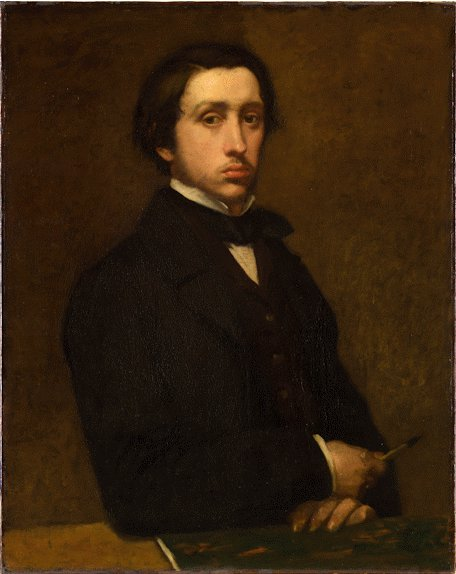
\includegraphics[scale=0.5]{Edgar_Degas_self_portrait_1855.jpeg}}
\end{frame}
\begin{frame}
  \centerline{
\includegraphics[scale=0.15]{DanielHaskin-small.jpg}}
  \center{
    Daniel Jay Haskin \\
    @djhaskin987
  }
\end{frame}
\begin{frame}[fragile]
  \centerline{\color{blue}\Large Dependencies Are The Worst}
\end{frame}
\begin{frame}
  \frametitle{Why Degasolv?}

  Does this sound like problems you deal with?

  \break

  \begin{itemize}
  \item Lots of first party dependencies within the product
  \item All (or lots) of the product's third-party dependencies are built on-site
  \item Some languages/technologies don't have a dependency manager
  \item Cross-technology dependencies
  \item Deal with site-specific quirks
  \end{itemize}

  \break

  Then degasolv may be for you.

\end{frame}
\begin{frame}
  \frametitle{Design Goals}
  \begin{itemize}
  \item Degasolv is designed specifically for use by build and DevOps engineers
  \item Degasolv is safe to use
  \item Degasolv is a ``stays out of your way''
  \item If Degasolv makes you angry, then there is a bug in Degasolv.
  \end{itemize}
\end{frame}
\begin{frame}
  \frametitle{Design Goals}
  \begin{itemize}
    \item Degasolv is a ``closed diamond'' resolver
  \end{itemize}
  \centerline{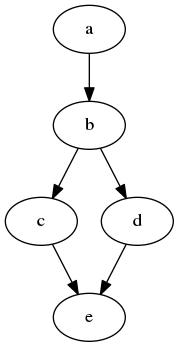
\includegraphics[scale=0.5]{diamonddep.png}}
\end{frame}
\begin{frame}
  \frametitle{Overview}
  \begin{itemize}
  \item \texttt{generate-card}: Generate a ``card file'' which represents a package
  \item Upload the card file to a NAS or other central file share
  \item \texttt{generate-repo-index}: Generate a ``repository index''
    based on the card files in the central file share
  \item \texttt{query-repo}: Inspect what packages exist in the repository
  \item \texttt{resolve-locations}: Using repository indices, find the locations
    of packages and their dependencies
  \end{itemize}
\end{frame}
\begin{frame}
  \frametitle{What is a Degasolv ``Package''?'}
  \begin{itemize}
  \item A name
  \item A version
  \item A URL
  \item A list of dependencies
  \end{itemize}
\end{frame}
\begin{frame}
  \frametitle{Requirement Syntax Overview}
  \begin{itemize}
  \item A "requirement" is a predicate describing a package, given as a string.
  \item Sort of its own mini language, but it should look familiar
  \item Given as a string
  \item Used in \texttt{generate-card} to specify dependencies
  \item Used in \texttt{resolve-locations} to specify what packages to resolve
  \item Subset of the language used in \texttt{query-repo} to query repository for
    matching packages
  \item Specify version ranges, version exceptions
  \item Supports boolean operators
  \item Consult the docs for more info
  \end{itemize}
\end{frame}
\begin{frame}[fragile]
  \frametitle{Requirement Syntax Examples}
\begin{verbatim}
    "oak"
    "pine>1.0"
    "hickory>1.0,<=2.0"
    "fir<=2.0;>3.5,!=3.8"
    "oak|pine>5.0"
    "hickory>=3.0,<4.0"
    "!birch|birch<=3.0", "!birch>3.0"
    "!oak|maple>3.0"
    "oak|!pine"
\end{verbatim}
\end{frame}
\begin{frame}
  \frametitle{\texttt{generate-card} Overview}
  \begin{itemize}
  \item Generates ``card'' files, which contain data about a particular package
  \item Keeps track of dependency information indepently of actual package file contents
  \item As a convention, it's good to name your dscard file after the file to which
    the URL points (e.g., \texttt{e-1.8.0.zip.dscard})
  \item Using card files as in place of actual build artifacts makes
    dependency resolution a completely independent part of your build; you
    don't have to ask developers to change the product to use it.
  \end{itemize}
\end{frame}
\begin{frame}[fragile]
  \frametitle{\texttt{generate-card} Example}
\begin{minted}{bash}
    java \
        -jar ./degasolv-1.0.3-SNAPSHOT-standalone.jar \
        generate-card \
        --id "d" \
        --version "0.8.0" \
        --location "https://example.com/repo/d-0.8.0.zip" \
        --requirement "e>=1.1.0,<2.0.0" \
        --card-file $PWD/d-0.8.0.zip.dscard
\end{minted}
\end{frame}
\begin{frame}[fragile]
  \frametitle{\texttt{generate-card} Output: The \texttt{*.dscard} File}
\begin{minted}{clojure}
    ; Filename: d-0.8.0.dscard
    #degasolv.resolver/PackageInfo {
        :id "d",
        :version "0.8.0", 
        :location "https://example.com/repo/d-0.8.0.zip", 
        :requirements [ [
            #degasolv.resolver/Requirement {
                :status :present,
                :id "e", 
                :spec [ [
                    #degasolv.resolver/VersionPredicate {
                        :relation :greater-equal, 
                        :version "1.1.0"}
                    #degasolv.resolver/VersionPredicate {
                        :relation :less-than,
                        :version "2.0.0"
                    }
                ]]
            }
        ]]
    }
\end{minted}
\end{frame}
\begin{frame}[fragile]
  \frametitle{\texttt{generate-card} Final Step: Deposit the Card File}
  \begin{itemize}
  \item After the card file is generated, it needs to be deposited into a
    central file share
  \end{itemize}
\begin{minted}{bash}
    $ find .
    .
    ./c-3.5.0.zip.dscard
    ./b-2.3.0.zip.dscard
    ./e-2.1.0.zip.dscard
    ./e-2.4.0.zip.dscard
    ./e-1.8.0.zip.dscard
    ./d-0.8.0.zip.dscard
    ./c-2.4.7.zip.dscard
\end{minted}
\end{frame}
\begin{frame}
  \centerline{\color{blue}\Large \texttt{generate-card} Demo}
\end{frame}
\begin{frame}
  \frametitle{\texttt{generate-repo-index} Overview}
  \begin{itemize}
  \item Patterned after YUM's \texttt{createrepo}
  \item Running \texttt{generate-repo-index} from the directory containing \texttt{*.dscard}
    files
  \item The index will then contain information about packages represented in those
    files
  \end{itemize}
\end{frame}
\begin{frame}[fragile]
  \frametitle{\texttt{generate-repo-index} Example}
\begin{minted}{bash}
    java \
        -jar ./degasolv-1.0.3-SNAPSHOT-standalone.jar \
        generate-repo-index \
        -d $PWD \
        -I $PWD/index.dsrepo
\end{minted}
\end{frame}
\begin{frame}[fragile]
  \frametitle{\texttt{generate-repo-index} Output}
\begin{minted}{bash}
    $ find .
    .
    ./c-3.5.0.zip.dscard
    ./b-2.3.0.zip.dscard
    ./e-2.1.0.zip.dscard
    ./e-2.4.0.zip.dscard
    ./e-1.8.0.zip.dscard
    ./d-0.8.0.zip.dscard
    ./c-2.4.7.zip.dscard
    ./index.dsrepo # <----- new file
\end{minted}
\end{frame}
\begin{frame}
  \centerline{\color{blue}\Large \texttt{generate-repo-index} Demo}
\end{frame}
\begin{frame}
  \frametitle{\texttt{resolve-locations} Overview}
  \begin{itemize}
  \item This command resolves dependencies given a target expression
  \item The names, versions, and URLs of the resolved packages are printed
  \item The output is designed to be both machine and human readable
  \item Command is designed to be used within build scripts
  \end{itemize}
\end{frame}
\begin{frame}[fragile]
  \frametitle{\texttt{resolve-locations} Example}
  Command:
\begin{minted}{bash}
    java \
        -jar ./degasolv-1.0.3-SNAPSHOT-standalone.jar \
        resolve-locations \
        -R $PWD/index.dsrepo \
        -r "b"
\end{minted}
  Output:
\begin{verbatim}
    c==3.5.0 @ https://example.com/repo/c-3.5.0.zip
    d==0.8.0 @ https://example.com/repo/d-0.8.0.zip
    e==1.8.0 @ https://example.com/repo/e-1.8.0.zip
    b==2.3.0 @ https://example.com/repo/b-2.3.0.zip
\end{verbatim}
\end{frame}
\begin{frame}
  \centerline{\color{blue}\Large \texttt{resolve-locations} Demo}
\end{frame}

\begin{frame}
  \frametitle{\texttt{query-repo} Overview}
  \begin{itemize}
  \item This command allows the user to query the repository index directly
  \item Implemented to allow the engineer to debug the build
  \end{itemize}
\end{frame}
\begin{frame}[fragile]
  \frametitle{\texttt{query-repo} Example}
  Command:
\begin{minted}{bash}
    java \
        -jar ./degasolv-1.0.3-SNAPSHOT-standalone.jar \
        --config-file $PWD/config.edn \
        query-repo \
        --query "e>2.0.0,!=2.1.0"
\end{minted}
  Output:
\begin{verbatim}
    e==2.4.0 @ https://example.com/repo/e-2.4.0.zip
\end{verbatim}
\end{frame}

\begin{frame}
  \centerline{\color{blue}\Large \texttt{query-repo} Demo}
\end{frame}
\begin{frame}
  % For this demo we will do multi-technology and native in the same demo,
  % Patterned after what I've seen before, but also patterned after the
  % 'Longer Example' I gave in the docs.
  \centerline{\color{blue}\Large Demo}
\end{frame}
\begin{frame}[fragile]
  \frametitle{JFrog Artifactory Integration}
  \begin{itemize}
  \item JFrog artifactory CLI already pairs well with degasolv
  \end{itemize}
\end{frame}
\begin{frame}[fragile]
\frametitle{JFrog Artifactory Integration: Setup}
\begin{minted}{bash}
    #!/bin/sh

    package_name="top"
    build_name="jenkins-${package_name}"
    build_number="18"

    jfrog rt build-clean "${build_name}" "${build_number}"
    jfrog rt build-collect-env "${build_name}" "${build_number}"
    jfrog rt build-add-git "${build_name}" "${build_number}"
\end{minted}
\end{frame}
\begin{frame}[fragile]
\frametitle{JFrog Artifactory Integration: Download}
\begin{minted}{bash}
    for dep in $(java \
        -jar ./degasolv-1.0.3-SNAPSHOT-standalone.jar \
        resolve-locations \
        --repository=<ARTIFACTORY-REPO-URL>/index.dsrepo \
        top_dep_a top_dep_b top_dep_c | \
        awk -F' *@ *' '{print $2}')
    do
        # In this example, the `dep` variable is of the form
        # <artifactory-repo>/<path-to-artifact>
        jfrog rt download \
            --build-name "${build_name}" \
            --build-number "${build_number}" \
            "${dep}"
            ./deps
    done
\end{minted}
\end{frame}
\begin{frame}[fragile]
\frametitle{JFrog Artifactory Integration: Upload}
\begin{minted}{bash}
    jfrog rt upload \
        --build-name "${build_name}" \
        --build-number "${build_number}" \
        ./target/<artifact> \
        <artifactory-repo>/<path-to-artifact>
    jfrog rt upload \
        --build-name "${build_name}" \
        --build-number "${build_number}" \
        ./target/<artifact>.dscard \
        <artifactory-degasolv-repo>/<path-to-card>.dscard
    jfrog rt build-publish "${build_name}" "${build_number}"

\end{minted}
\end{frame}
\begin{frame}
  \frametitle{JFrog Artifactory Integration: Result}
  \begin{itemize}
  \item Build information for your artifact is published
  \item Artifacts that were downloaded via \texttt{jfrog rt download} are listed as
    dependencies to the artifacts uploaded via \texttt{jfrog rt upload} in the build
    information
  \end{itemize}
\end{frame}
\begin{frame}
  \frametitle{Summary}
\end{frame}
\begin{frame}
  \frametitle{Community}
  \textit{To use a thing, join its people.}

  \break

  \begin{itemize}
  \item Gitter room ``degasolv'' \\
    {\small https://gitter.im/degasolv/Lobby}
  \item Google group ``degasolv-users'' \\
    {\small https://groups.google.com/forum/\#!forum/degasolv-users}
  \end{itemize}
\end{frame}
\begin{frame}
  \frametitle{Future Directions}
  \begin{itemize}
  \item JFrog Artifactory plugin
  \item Resolution directly from different types of repositories
  \item Homebrew \\
    {\small https://github.com/Homebrew/brew/blob/master/docs/Formula-Cookbook.md}
  \item RPM, Debian packages
  \end{itemize}
\end{frame}
\begin{frame}
  \frametitle{Further Reading}
  \begin{itemize}
  \item Kill Your Dependencies {\small http://www.mikeperham.com/2016/02/09/kill-your-dependencies/}
  \item Embracing Conway's Law {\small https://wingolog.org/archives/2015/11/09/embracing-conways-law}
  \item JFrog Artifactory CLI {\small https://www.jfrog.com/confluence/display/CLI/CLI+for+JFrog+Artifactory}
  \end{itemize}
\end{frame}
\begin{frame}
  \centerline{\color{blue}\Large Questions}
\end{frame}
\end{document}
